Nous essayons d'être au maximum pro-actif vis à vis de notre projet en identifiant au maximum les risques prossibles
et en essayant de les prévenir. Pour ce faire, nous nous sommes réunis durant la première période du planning pour faire
un "brainstorming" pour identifier les risques liés à ce projet. Nous avons aussi aprés quelques réunions clients ajouté des risques
liés au client. Au final, pour identifier les risques, nous avons divisé en deux notre domaine de recherche : l'un concerne 
les clients et les spécifications, l'autre le programme ou tout ce qui est lié au code.	Pour identifier les risques, nous avons essayer d'imaginer la
démarche que l'on allait suivre pour terminer ce projet, et à chaque jalon important, on a essayé d'imaginer les problèmes qui pourrait survenir. 


	Par exemple, nous avons identifié un risque important aprés les quelques réunions clients que nous avons eu. L'un de nos 
client n'avait pas l'air trés sur ce qu'il attendait de nous. Nous avons appelé ce risque dans le tableau suivant "Client changes his mind". 
Ceci peut en effet complétement retarder la seconde partie dans le planning : le développement. Nous avons essayé de prévenir et résoudre 
ce risque en utilisant la technique des "5 Why" :\\
\begin{itemize}
\item Pourquoi le client changerait ce que nous étions entrain de faire ? Parce qu'il a changé d'avis.\\
\item  Pourquoi ? Parce que nous n'avions pas été clair lors de la réunion précédente.\\
\item Pourquoi ? Parce que nos spécifications ne sont pas claires et/ou pas bien rédigées dans le cahier des spécifications.\\
\item Pourquoi ? Parce que nous devons faire signer une fois pour toute les spécifications par ce client. Ainsi il ne pourra plus changer.\\
\end{itemize}

Nous avons ainsi prévenu ce problème en faisant, bien que un peu tard, signer les spécifications. Nous avons tout de même associé à ce risque
une probabilité d'apparition importante et un impact important sur le développement, comme indiqué dans le tableau ci dessous. 


	Un autre risque, cette fois lié au code, est que la bibliothèque openMVG soit trop lente pour permettre une reconstruction rapide. Notre
programme doit être utilisé dans l'industrie du cinéma, et si il faut un mois pour reconstruire une scène, cela n'a pas trop d'interêt. Hors la lenteur
vient de openMVG, et nous devons utiliser cette bibliothèque. On ne peut donc pas prévenir ce rique, qui a tout de même une probabilité moyenne
d'apparaître et un impact sur le résultat et le développement (en effet nous serons donc peut être amener à modifier openMVG) importante.


	Enfin un dernier risque que nous détaillerons ici est celui associé au fait que l'on ne puisse pas relancer une nouvelle reconstruction
à partir d'une déjà existante. Ce risque a une probabilité peu importante d'apparaître et un impact moyen sur le développement. En effet,
l'un de nos client nosu a assuré qu'il pourrait modifié la bibliothèque pour permettre ceci.


	Les autres risques sont présentés dans le tableau ci dessous, ainsi que leur probabilité d'apparition et leur impact sur le projet. 

\begin{figure}
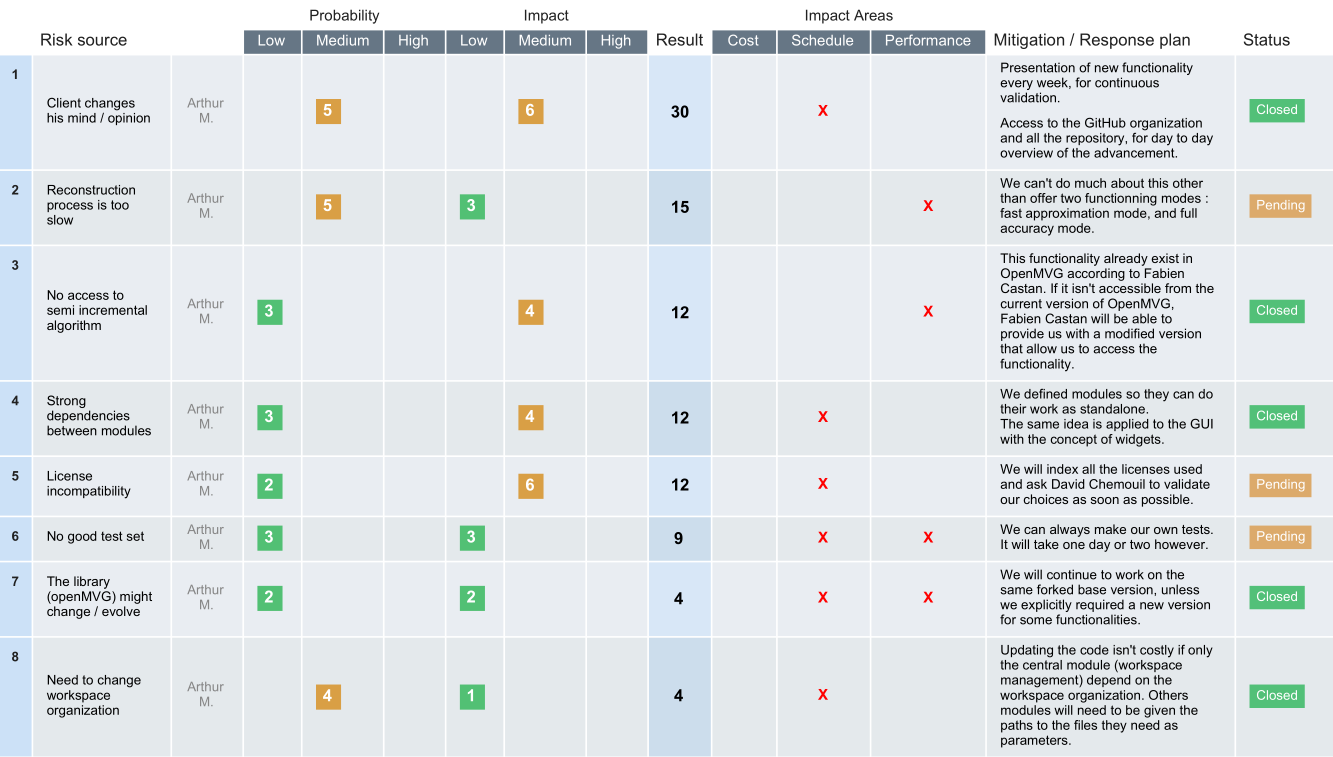
\includegraphics[scale=0.48]{risques.png}
\end{figure}	
